\documentclass[12pt]{article}

\usepackage{graphicx}

\graphicspath{{./images/}}

\title{Assignment 2 2ME3}
\author{Aryaan Sheth}
\date{Nov 17, 2022}

\begin{document}
    \maketitle
    \newpage

    \part{}
    \section*{UML Diagram of Design}
        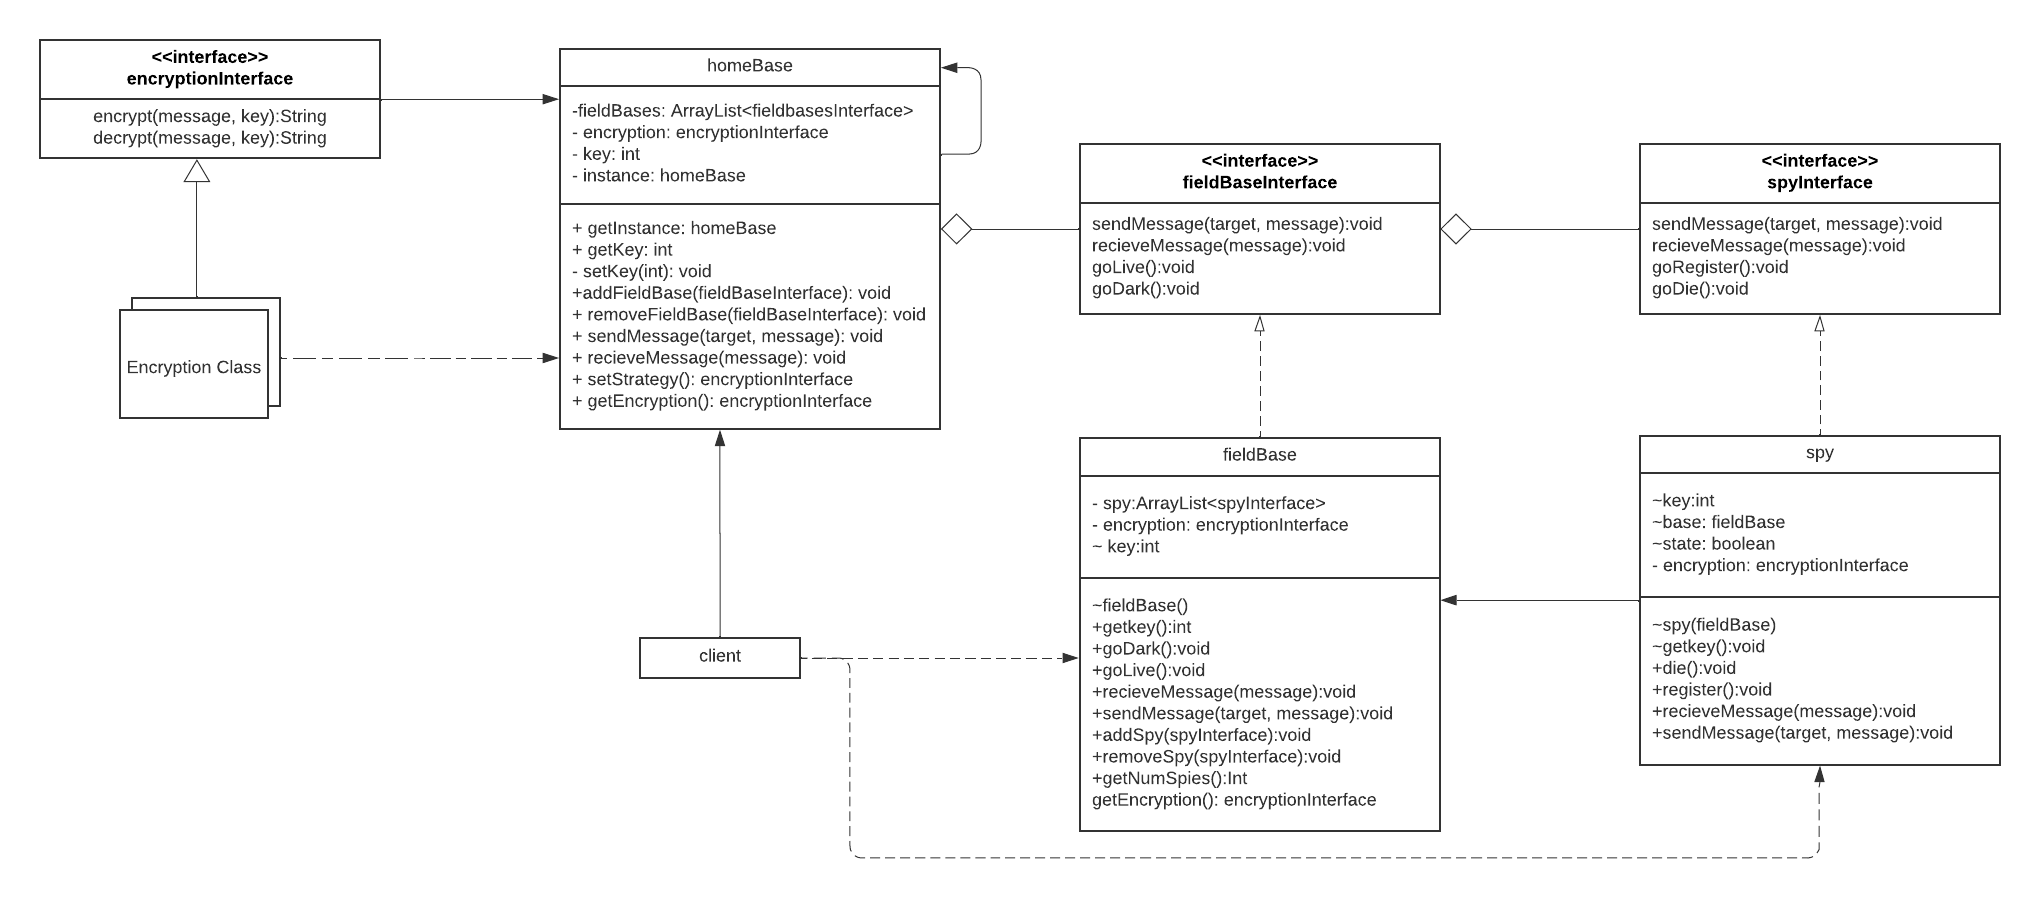
\includegraphics[scale=.25]{part1_uml}

    \section*{Design Patterns}
        \subsection*{Encryption}
            For the multiple encryption schemes that our design needs to support, I used the \textbf{Strategy}
            pattern as it allowed me to easily swap in and out different behaviors for the encryption schemes.
            It also allowed to change encryption schemes on the go using setters in the Home Base. 

        \subsection*{Home Base}
            For the home base, I chose to use the \textbf{singleton} design pattern. This is because
            the instructions document emphasized the importance of having only one home base. The singleton
            pattern does exactly that and limits the number of instances of the class to one. 
            This is done by checking the existence of the class in its constructor and only instantiating a new
            instance of that class the class was initialized to null. 
        
        \subsection*{Field Base \& Spy}
            For both these classes, I chose to use a \textbf{observer} design pattern. The main reason was for the messaging feature
            and wanting all other classes to be able to send messages to each other. The observer pattern allows
            for this to happen. Both the field base and spy classes are built from an interface which allows multiple instance
            of the class to be created easily. 

        \subsection*{Future Thoughts}
            If we wanted to implement a system to ship out multiple home bases around to different locations, we 
            could use the \textbf{factory} design pattern. This would allow us to create multiple 
            instances of the home base that come pre-packaged with field bases and spies. To achieve
            this we would create a wrapper class of the current structure and apply the factory pattern on that. 
    \section*{Design Principals}
        \subsection*{DRY}
            My design follows the DRY principle as I use interfaces, abstract classes, and generics to reduce 
            the amount of code that needs to be re-written in the code. For example, the 
            bitshift and decryption methods are implemented in the abstract class and all the classes
            can call on that which reduces the amount of code that needs to be written within the individual classes. 
        \subsection*{Open-Close Principal}
            My design follows the open close principal as it's very modular and it is super easy to add new features 
            and functions to classes via the use of the interfaces and abstract classes that encompass the structure. 
            For example, if we wanted to add a new type of spy that can do something different, we can simply create a 
            new spy that extends the spy class and implement the new methods that are needed.
        \subsection*{Design For Interfaces}
            My design follows the design for interfaces principal as all the classes are built from interfaces and their structure is
            dictated by the interface. For example, the spies and field bases are built from the spy and field base interfaces
            which dictate the structure of the classes such as their goLive and goDark methods. 

    \section*{Design Intention}
        My design intention is to create a modular design that allows for easy expansion on existing classes via child classes or using 
        a design pattern such as factory to create multiple instances of the home base design. This is done by using interfaces
        to create a structure that can be easily expanded on. With the use of the observer pattern, we can easily add new classes and chain them together to create a new 
        subsystem from field bases and agent and expand the overall structure. This also enables the messaging system to work as it allows for the classes to
         be able to send messages to each other and the home base and be notified of them. 

    \part{}
    \section*{UML Diagram of New Design}
        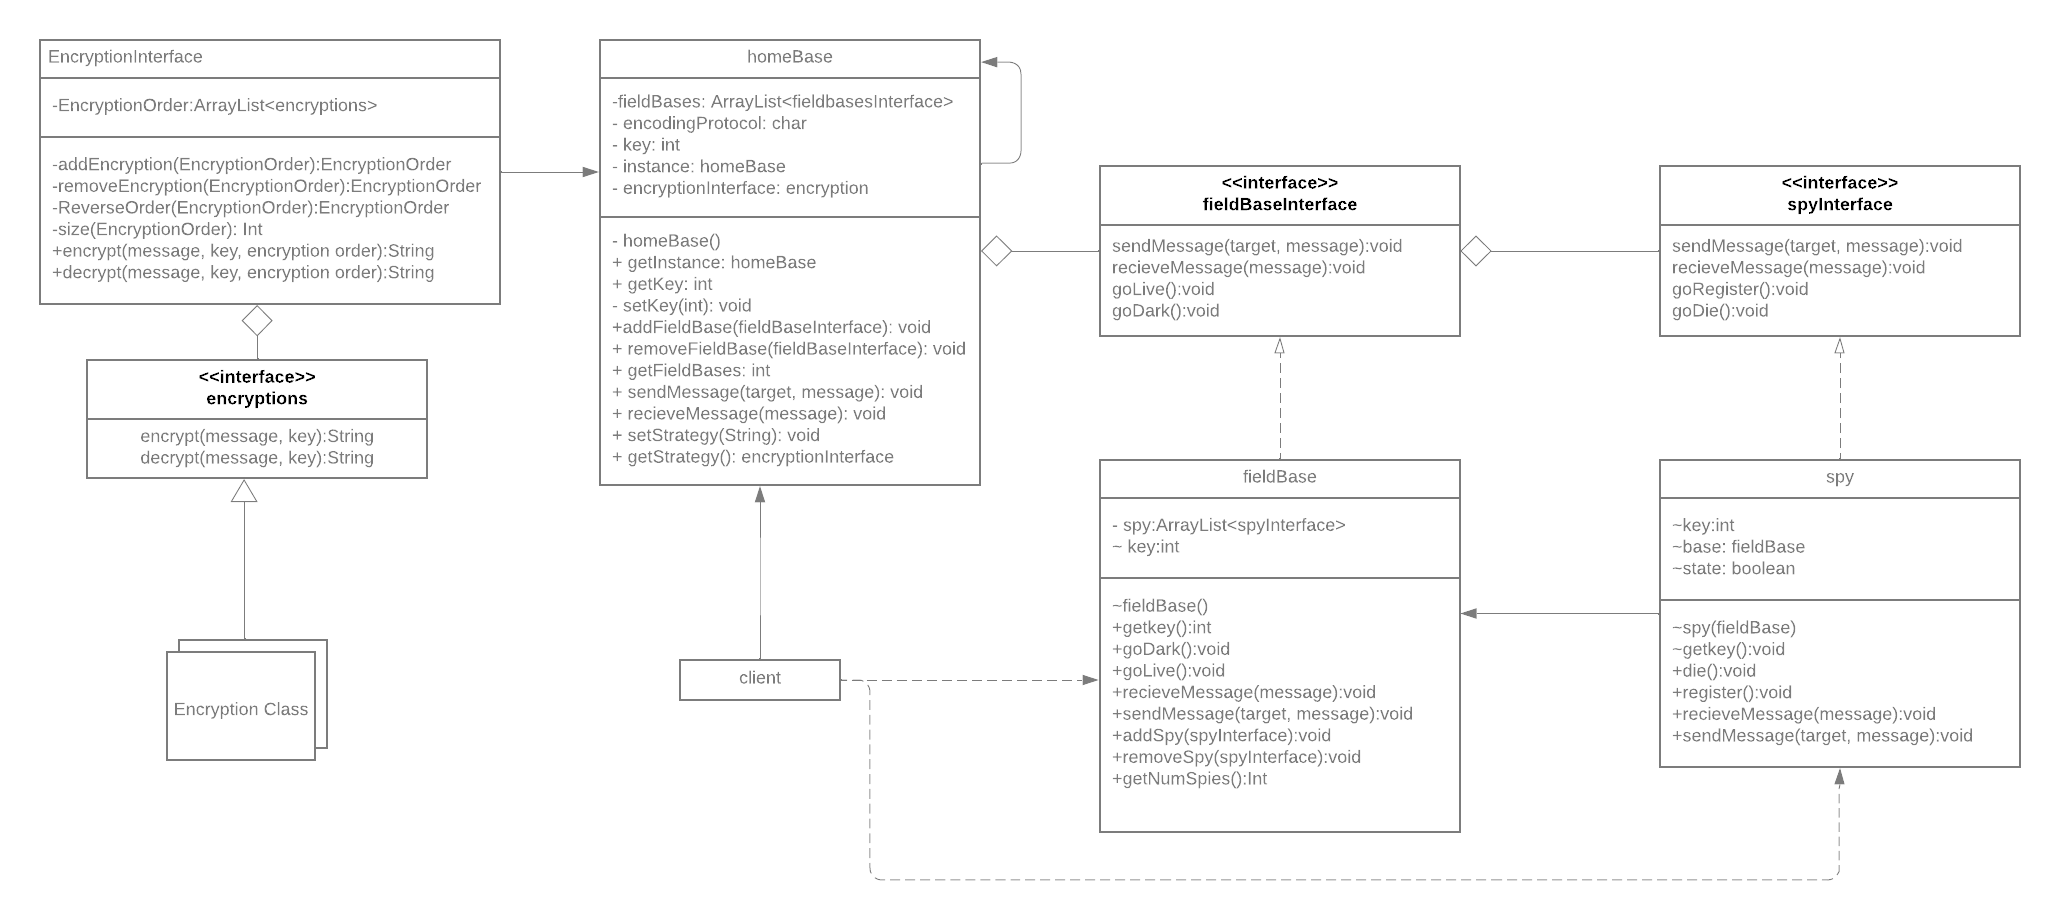
\includegraphics[scale=.24]{part2_uml}
    
    \section*{Modification Of Program}
        With the updated UML, the new encryption interface is an interface between the actual interface and the concrete
        homeBase class. It extends the functionality of the current encryption logic and allows for the home base to be able to
        multiple layers of encryption. This is done by updating the call methods in the homeBase to call the new 
        encryption function which will give it access to adding multiple encryption layers using an ArrayList. 
        
\end{document}